\documentclass{article}
\usepackage[utf8]{inputenc}
\usepackage{xcolor}
\usepackage{graphicx}
\usepackage{listings}

\definecolor{codegreen}{rgb}{0,0.6,0}
\definecolor{codegray}{rgb}{0.5,0.5,0.5}
\definecolor{codepurple}{rgb}{0.58,0,0.82}
\definecolor{backcolour}{rgb}{0.95,0.95,0.92}

\lstdefinestyle{mystyle}{
    backgroundcolor=\color{backcolour},   
    commentstyle=\color{codegreen},
    keywordstyle=\color{magenta},
    numberstyle=\tiny\color{codegray},
    stringstyle=\color{codepurple},
    basicstyle=\ttfamily\footnotesize,
    breakatwhitespace=false,         
    breaklines=true,                 
    captionpos=b,                    
    keepspaces=true,                 
    numbers=left,                    
    numbersep=5pt,                  
    showspaces=false,                
    showstringspaces=false,
    showtabs=false,                  
    tabsize=2
}

\lstset{style=mystyle}

\title{\color{blue}{ASSIGNMENT 3}}
\author{\Large{\texttt{NAME: \color{red}{Shafikha Yasmeen}      \color{black}{ID}:\color{red}{B192241}}}}

\begin{document}
\maketitle
\hrule
\vspace{1cm}
\Large\color{black}{DATA: }
\begin{figure}[h]
   \centering
    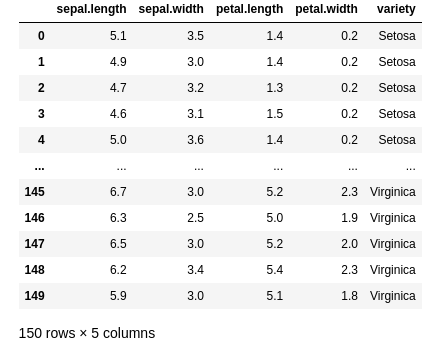
\includegraphics[width=1.1\textwidth]{Data.png}
\end{figure}
\newpage
\Huge{Reading the Data}
\Huge\lstinputlisting[language=Python]{intro.py}
\vspace{1cm}

\Huge\textbf{1.Pie Chart}
\Large\lstinputlisting[language=Python]{#1.py}
\begin{figure}[h]
    \centering
    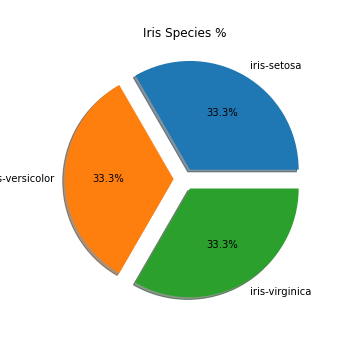
\includegraphics[width=0.7\textwidth]{1.png}
\end{figure}
\newpage

\Huge\textbf{2.Scatter Plot}
\Large\lstinputlisting[language=Python]{#2.py}
\vspace{10}
\begin{figure}[h]
   \centering
    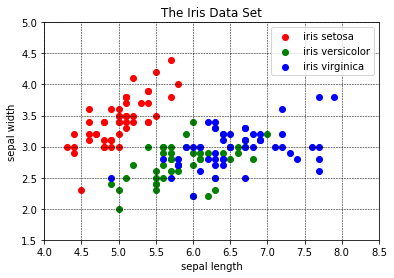
\includegraphics[width=0.9\textwidth]{2.png}
\end{figure}
\newpage

\Huge\textbf{3.Bar Graph}
\vspace{2cm}
\Large\lstinputlisting[language=Python]{#3.py}
\newpage


\begin{figure}[h]
   \centering
   \vspace{1cm}
    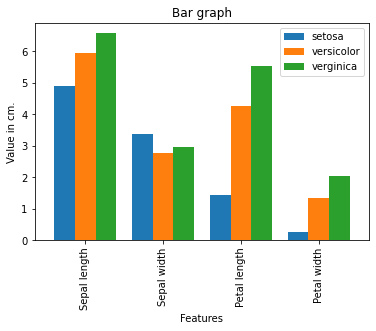
\includegraphics[width=1.3\textwidth]{3.png}
\end{figure}
\newpage


\Huge\textbf{4.Iris Histograms}
\vspace{3cm}
\Large\lstinputlisting[language=Python]{#4.py}
\begin{figure}[h]
\centering
    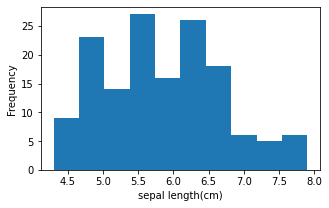
\includegraphics[width=0.7\textwidth]{4.1.png}\\
    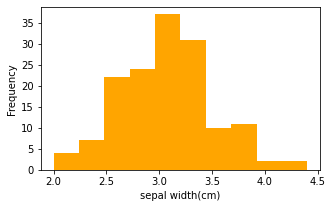
\includegraphics[width=0.7\textwidth]{4.2.png}\\
    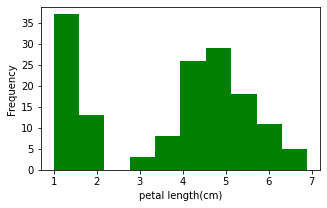
\includegraphics[width=0.7\textwidth]{4.3.png}\\
    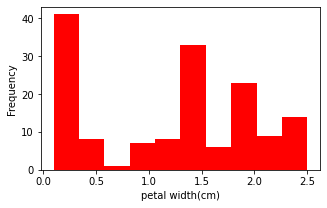
\includegraphics[width=0.7\textwidth]{4.4.png}\\
    
\end{figure}
\end{document}